\chapter{Problem statement and formulation}\label{ch:problem-statement-and-formulation}

This chapter defines the painting placement problem, its inputs, constraints, and what a solution to the painting placement problem is.
First, let us define what a painting placement instance is.\\

\navesti{Painting placement isntance} is an ordered quadruple

\begin{equation}
    I = (P, F, L, \pi)\,,
    \label{eq:painting-placement-instance}
\end{equation}

where $P \subseteq (\nat, \nat)^N$ are painting dimensions (width, height pairs),
$N$ is the number of paintings,
$F \subseteq \real^{N, N}$ is matrix defining flow between paintings,
$L \in (\nat, \nat)$ is layout dimension (width, height pair)
and $\pi: \real \times \real \to \real$ is evaluation function.

Flow expresses the affinity of paintings to each other.
Paintings that should be placed close together have flow higher compared to paintings
that should not.
Additionally, layout and painting dimensions are abstract, e.g., they have dimensionless units.
However, they can be interpreted as any suitable measurement unit, e.g., meters.


An example of a painting placement instance is

\[
    I_1 = (\overbrace{\langle (5,4),(8,5) \rangle}^{paintings},
    \overbrace{\begin{pmatrix}
                   0   & 5.8 \\
                   5.8 & 0
    \end{pmatrix}}^{flow},
    \overbrace{(15,7)}^{layout},
    \overbrace{f(x,y) = x+y)}^{evaluation function}\,.
\]

Instance $I_1$ contains two paintings, the first with dimensions $5\times4$, the second with $8\times5$.
The flow between them is $5.8$.
The layout to which paintings are placed has a width $15$ and a height $7$.
The evaluation function is $x+y$.

Next, each painting placement instance can have multiple solutions.\\

\navesti{Painting placement solution} is a sequence of placement points
\begin{equation}
    S \subseteq (\nat,\nat)^N  \,.
    \label{eq:painting-placement-solution}
\end{equation}

For example, one solution $S_1$ for the instance $I_1$ is

\[
    S_1 = \langle (0,0), (6,1) \rangle \,.
\]

It means that the first painting's lower left corner has coordinates $(0,0)$
and similarly $(6,1)$ for the second painting.
Illustration of both $I_1$ and $S_1$ can be seen in figure~\ref{fig:painting-placement-solution}.

\begin{figure}
    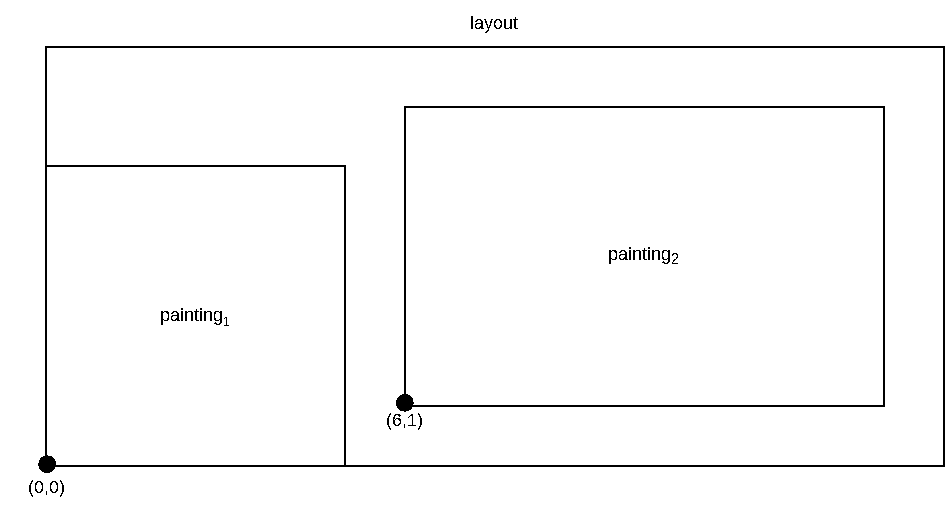
\includegraphics[width=0.9\textwidth, left]{painting_placement_solution}
    \caption[Example of a painting placement solution]{Example of a painting placement solution $S_1 = \langle (0,0), (6,1) \rangle$ for instance $I_1$.}
    \label{fig:painting-placement-solution}
\end{figure}

\newpage

Lastly, we need to evaluate the performance of the painting placement solution.
Let us assume a painting placement instance $I$ and a set of all possible painting placement solutions $S$ to that instance.
Then, the \definice{painting placement problem} is to find a minimum of a cost function $c: S \to \realpos$,
which can also be called an objective function, as


\begin{equation}
    \argmin_{x \in S} c(x) = \sum\limits_{i=1}^N\sum\limits_{j=i+1}^N f_{i,j}d(i, j) + \sum\limits_{i=1}^N \pi(i) + \lambda m(x) + \gamma n(x) \,,
    \label{eq:objective}
\end{equation}

where $f_{i,j}$ is flow between painting $i$ and $j$, $d(i,j)$ is their distance,
$\pi(i)$ is the evaluation function applied to the bottom left corner of the painting's $i$  placement point,
$m$ calculates number of overlapping paintings with penalization constant $\lambda \in \real^+$
and $n$ calculates the number of paintings placed outside their allocated area (see~\ref{subsec:placement-heuristic})
with penalization constant $\gamma \in \real^+$.

The problem defined as such is NP-hard.
The reason is that by setting penalization constants $\lambda$, $\gamma$ to zero and $\pi$ to $f(x,y) = 0$,
the objective function of a painting placement problem becomes similar to the FLP objective as defined in equation~\ref{eq:flp-objective}.
The only difference is the price for a unit of distance in the FLP objective, but it can be added to the flow making the objective functions identical.
Also, at FLP, placed facilities are defined in terms of their area and maximum aspect ratio as opposed to width and height pair in the painting placement problem.
However, the facilities at the FLP problem must be assigned a dimension as the objective function application includes calculating the distance from placement points.
Thus, by FLP being NP-hard~\cite{liuMultiobjectiveParticleSwarm2018, goncalvesBiasedRandomkeyGenetic2015, friedrichIntegratedSlicingTree2018}, painting placement is also NP-hard.
